\documentclass[12pt]{article}
\usepackage[T1]{fontenc}
\usepackage[polish]{babel}
\usepackage[utf8]{inputenc}
\newcommand{\BibTeX}{{\sc Bib}\TeX}
\usepackage{graphicx}
\usepackage{amsfonts}
\usepackage[hidelinks]{hyperref}
\usepackage{float}
\usepackage{amsmath}

\usepackage{xcolor}
\usepackage{listings}
\lstset{
	basicstyle=\ttfamily\small,
	keywordstyle=\color{blue},
	commentstyle=\color{gray},
	stringstyle=\color{green!50!black},
	backgroundcolor=\color{black!5},
	showstringspaces=false,
	breaklines=true,
	frame=single,
	columns=flexible,
	keepspaces=true
}

\setlength{\textheight}{21cm}

\title{{\bf Zadanie nr 4 - Szybka transformacja Fouriera i transformacja falkowa}\linebreak
	Cyfrowe Przetwarzanie Sygnałów}
\author{Bartosz Kołaciński, 251554 \and Jakub Rosiak, 251620}
\date{\today}

\begin{document}
	\clearpage\maketitle
	\thispagestyle{empty}
	\newpage
	\setcounter{page}{1}

	\section{Cel zadania}
	Celem zadania jest implementacja oraz weryfikacja poprawności działania algorytmów szybkich transformacji: Fouriera (FFT) z decymacją w czasie i w częstotliwości, oraz dyskretnej transformacji falkowej (DWT). Analizie poddana została także złożoność obliczeniowa zaimplementowanych rozwiązań w porównaniu do transformacji wyznaczanych bezpośrednio z definicji.

	\section{Wstęp teoretyczny}
	Dyskretna Transformacja Fouriera (DFT) dla sygnału $x[n]$ o długości $N$ definiowana jest wzorem:
	\begin{equation}
		X[k] = \sum_{n=0}^{N-1} x[n] e^{-j\frac{2\pi}{N}kn}, \quad k = 0, \dots, N-1
	\end{equation}
	Bezpośrednie obliczenie DFT wymaga złożoności $O(N^2)$. Algorytmy FFT (Fast Fourier Transform) redukują tę złożoność do $O(N \log_2 N)$ poprzez rekurencyjny podział problemu (metoda „dziel i zwyciężaj”). Wyróżniamy m.in. decymację w czasie (DIT) oraz w częstotliwości (DIF).

	Transformacja falkowa (DWT) pozwala na analizę sygnału w dziedzinie czasu i częstotliwości jednocześnie. Wykorzystuje ona zestawy filtrów dolnoprzepustowych ($H$) i górnoprzepustowych ($G$). W zadaniu wykorzystano falki Daubechies (Db4 i Db6), które charakteryzują się zwartym nośnikiem i określoną liczbą momentów zerowych.

\section{Eksperymenty i wyniki}

Wszystkie eksperymenty przeprowadzono dla częstotliwości próbkowania $f_{pr} = 16\ \text{Hz}$.

\subsection{Prezentacja wygenerowanych sygnałów testowych}

Zgodnie z instrukcją wygenerowano trzy typy sygnałów testowych:
\begin{itemize}
    \item \textbf{S1}: Szum o rozkładzie jednostajnym w przedziale $[-A, A]$.
    \item \textbf{S2}: Szum o rozkładzie Gaussa o średniej 0 i odchyleniu standardowym $\sigma = A/3$.
    \item \textbf{S3}: Sygnał sinusoidalny $y(t) = A \sin(\frac{2\pi}{T}t)$.
\end{itemize}

Na rysunkach \ref{fig:s1}, \ref{fig:s2} i \ref{fig:s3} przedstawiono przebiegi czasowe tych sygnałów dla $N=32$ próbek.

\begin{figure}[H]
    \centering
    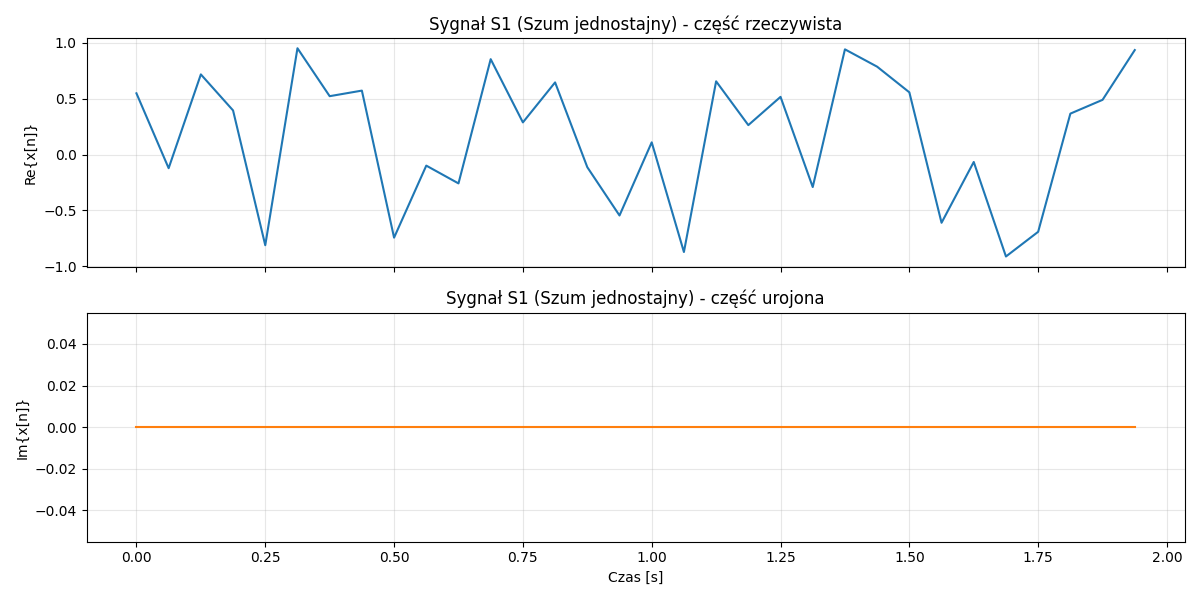
\includegraphics[width=0.8\textwidth]{img/signal_s1.png}
    \caption{Sygnał testowy S1 - szum jednostajny.}
    \label{fig:s1}
\end{figure}

\begin{figure}[H]
    \centering
    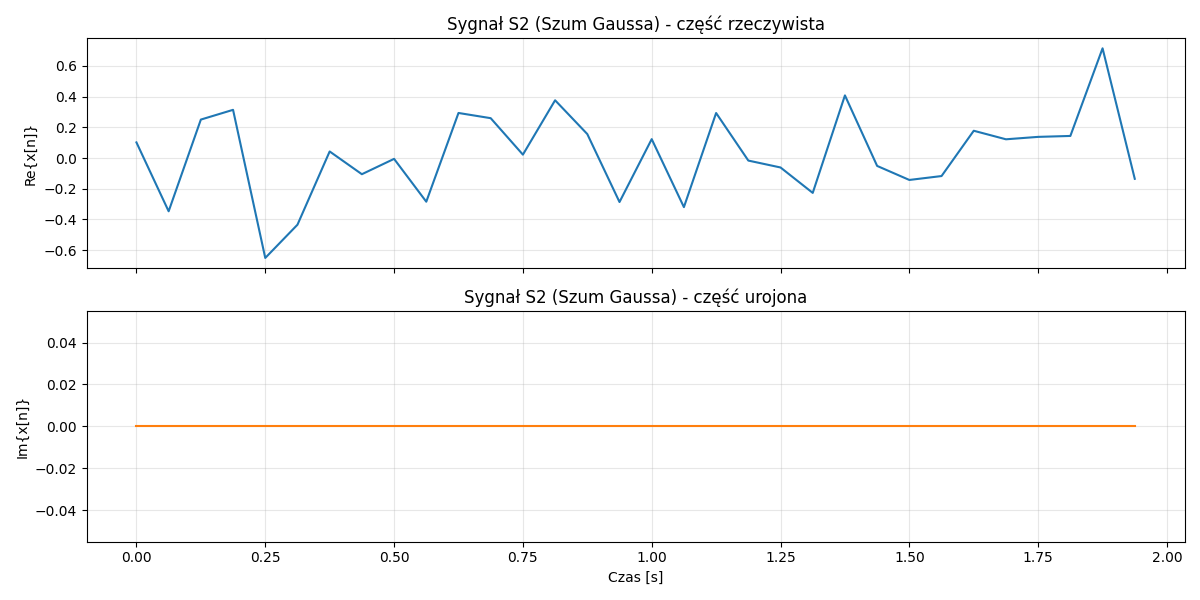
\includegraphics[width=0.8\textwidth]{img/signal_s2.png}
    \caption{Sygnał testowy S2 - szum Gaussa.}
    \label{fig:s2}
\end{figure}

\begin{figure}[H]
    \centering
    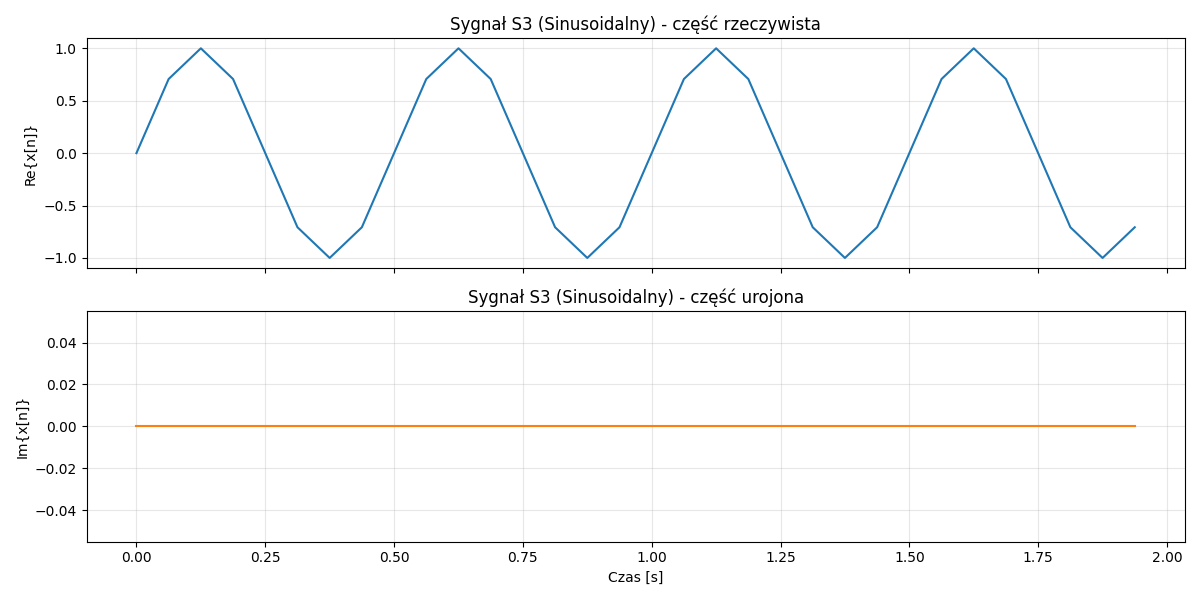
\includegraphics[width=0.8\textwidth]{img/signal_s3.png}
    \caption{Sygnał testowy S3 - sinusoida.}
    \label{fig:s3}
\end{figure}

\subsection{Weryfikacja transformacji Fouriera}

\textbf{Sprawdzenie poprawności (FFT2t i FFT2f):}
Zaimplementowane algorytmy \texttt{fft\_dit} (FFT2t) oraz \texttt{fft\_dif} (FFT2f) zostały zestawione z wynikami klasycznej transformacji DFT obliczanej z definicji dla sygnału zespolonego. Uzyskane błędy maksymalne są rzędu $10^{-14}$, co potwierdza poprawność implementacji w granicach precyzji zmiennoprzecinkowej.

\begin{table}[H]
    \centering
    \caption{Błąd maksymalny FFT względem DFT (definicja)}
    \begin{tabular}{|l|r|}
        \hline
        Algorytm & Max błąd bezwzględny \\
        \hline
        FFT DIT (Decymacja w czasie) & $5.74 \cdot 10^{-14}$ \\
        FFT DIF (Decymacja w częstotliwości) & $5.56 \cdot 10^{-14}$ \\
        \hline
    \end{tabular}
\end{table}

\textbf{Transformacja w miejscu i IDFT:}
Wykonano szybką transformację w przód, a następnie odwrotną (IFFT). Na rysunku \ref{fig:fft_rec} pokazano idealne odtworzenie sygnału wejściowego (błąd rzędu $10^{-16}$).

\begin{figure}[H]
    \centering
    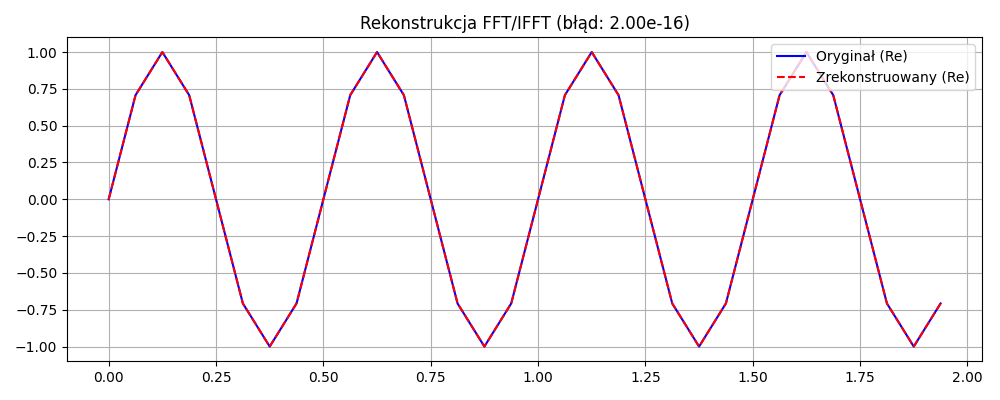
\includegraphics[width=0.8\textwidth]{img/fft_reconstruction.png}
    \caption{Rekonstrukcja sygnału po przejściu FFT i IFFT.}
    \label{fig:fft_rec}
\end{figure}

\textbf{Wizualizacja widma:}
Zaprezentowano transformaty sygnału w dwóch trybach: (W1) część rzeczywista i urojona (Rys. \ref{fig:spec_w1}) oraz (W2) moduł i faza (Rys. \ref{fig:spec_w2}).

\begin{figure}[H]
    \centering
    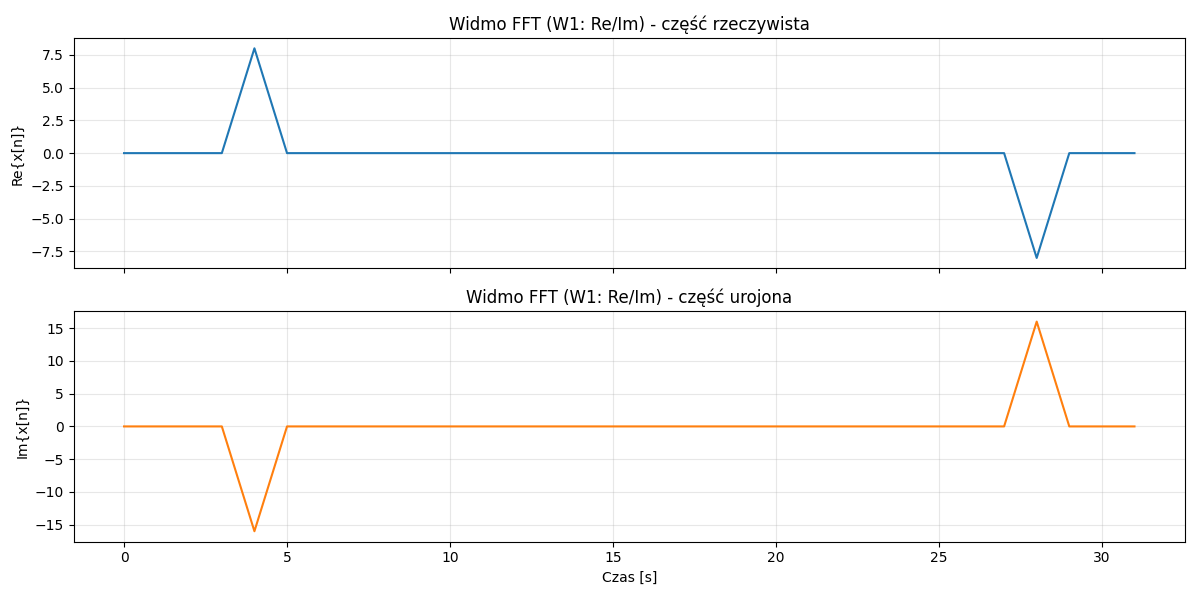
\includegraphics[width=0.8\textwidth]{img/spectrum_w1.png}
    \caption{Widmo sygnału - tryb W1 (część rzeczywista i urojona).}
    \label{fig:spec_w1}
\end{figure}

\begin{figure}[H]
    \centering
    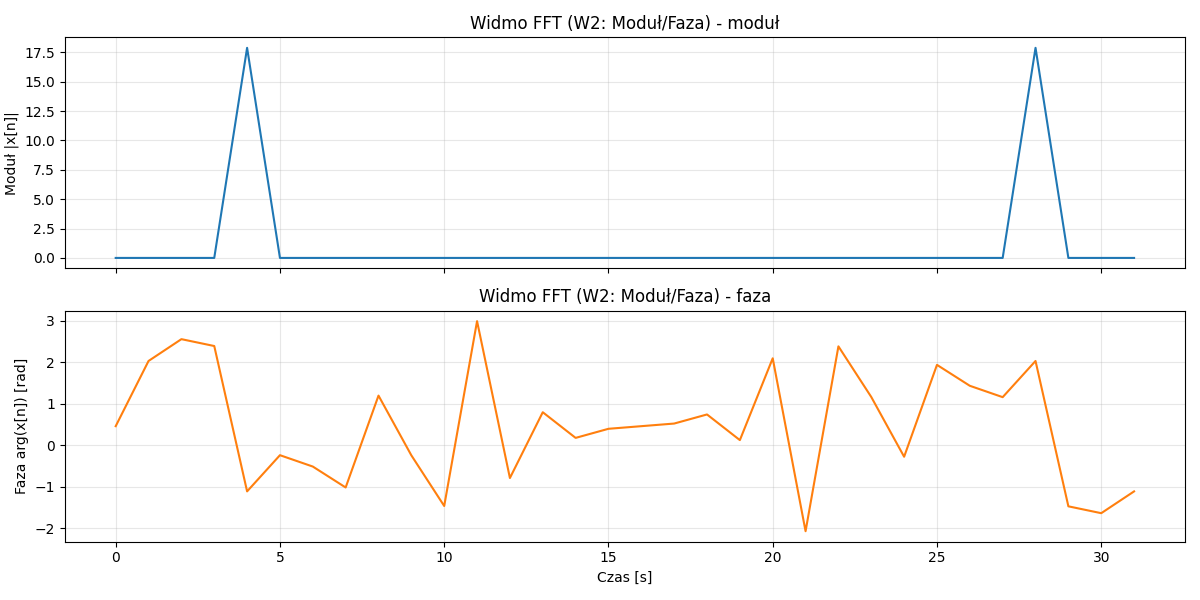
\includegraphics[width=0.8\textwidth]{img/spectrum_w2.png}
    \caption{Widmo sygnału - tryb W2 (moduł i faza).}
    \label{fig:spec_w2}
\end{figure}

\subsection{Weryfikacja transformacji falkowej (DWT)}

\textbf{Transformacja prosta i testy filtrów:}
Zastosowano falki Daubechies rzędu 4 i 6. Wykorzystano periodyczne rozszerzenie sygnału. Współczynniki filtrów analizy ($H$ - dolnoprzepustowy, $G$ - górnoprzepustowy) dla Db4 wynoszą:
\begin{lstlisting}
H: [-0.0106, 0.0329, 0.0308, -0.1870, -0.0280, 0.6309, 0.7148, 0.2304]
G: [ 0.2304, -0.7148, 0.6309, 0.0280, -0.1870, -0.0308, 0.0329, 0.0106]
\end{lstlisting}
Proces filtracji polega na splotach kołowych z przeskokiem (downsampling). Poprawność przejścia „na piechotę” zweryfikowano dla krótkich wektorów testowych, sprawdzając czy energia sygnału jest zachowana i czy filtry poprawnie separują pasma.

\textbf{Test idealnej rekonstrukcji:}
Na rysunkach \ref{fig:dwt_db4} i \ref{fig:dwt_db6} przedstawiono dowód na idealną rekonstrukcję sygnału po wykonaniu prostej i odwrotnej transformacji falkowej.

\begin{figure}[H]
    \centering
    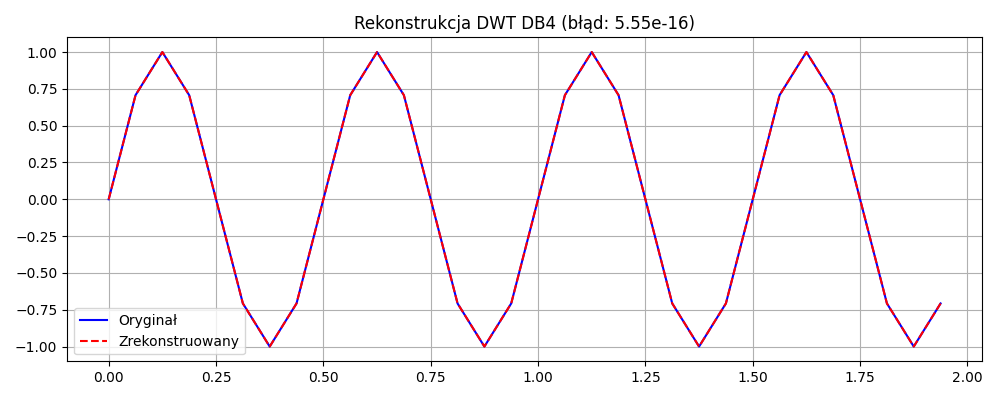
\includegraphics[width=0.8\textwidth]{img/dwt_db4_reconstruction.png}
    \caption{Idealna rekonstrukcja DWT Db4.}
    \label{fig:dwt_db4}
\end{figure}

\begin{figure}[H]
    \centering
    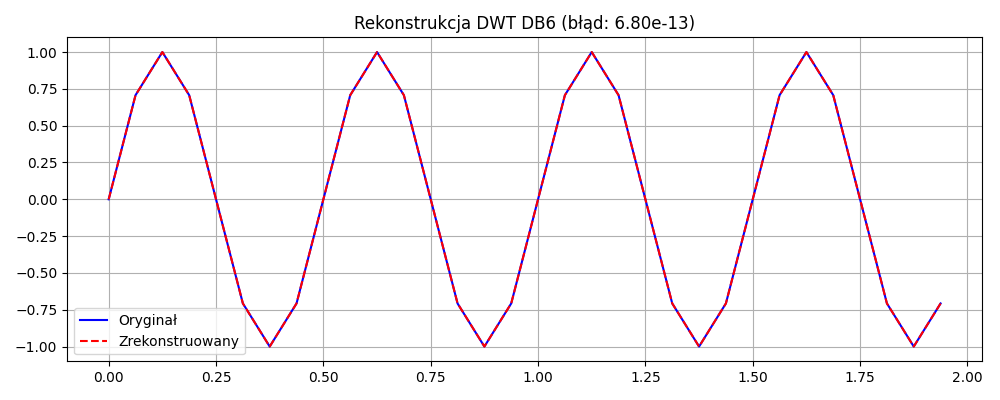
\includegraphics[width=0.8\textwidth]{img/dwt_db6_reconstruction.png}
    \caption{Idealna rekonstrukcja DWT Db6.}
    \label{fig:dwt_db6}
\end{figure}

\subsection{Pomiary czasu i analiza złożoności}

Przeprowadzono testy szybkości dla $N = 2^n$ ($n \in [1, 10]$). Wyniki zestawiono w tabeli \ref{tab:bench} oraz na wykresie \ref{fig:bench}.

\begin{table}[H]
    \centering
    \caption{Porównanie czasu wykonania transformacji [ms]}
    \label{tab:bench}
    \begin{tabular}{|r|r|r|r|r|}
        \hline
        N & DFT ($O(N^2)$) & FFT DIT & FFT DIF & NumPy FFT \\
        \hline
        2 & 0.0090 & 0.0076 & 0.0063 & 1.3970 \\
        4 & 0.0156 & 0.0107 & 0.0094 & 0.0086 \\
        8 & 0.0519 & 0.0189 & 0.0181 & 0.0639 \\
        16 & 0.1811 & 0.0393 & 0.0370 & 0.0093 \\
        32 & 0.6655 & 0.1139 & 0.1155 & 0.0111 \\
        64 & 3.3605 & 0.1897 & 0.2164 & 0.0171 \\
        128 & 12.6586 & 0.4370 & 0.5628 & 0.0246 \\
        256 & 50.0428 & 1.0323 & 1.1430 & 0.0145 \\
        512 & - & 2.4326 & 2.6331 & 0.0236 \\
        1024 & - & 5.1995 & 5.9518 & 0.0392 \\
        \hline
    \end{tabular}
\end{table}

\begin{figure}[H]
    \centering
    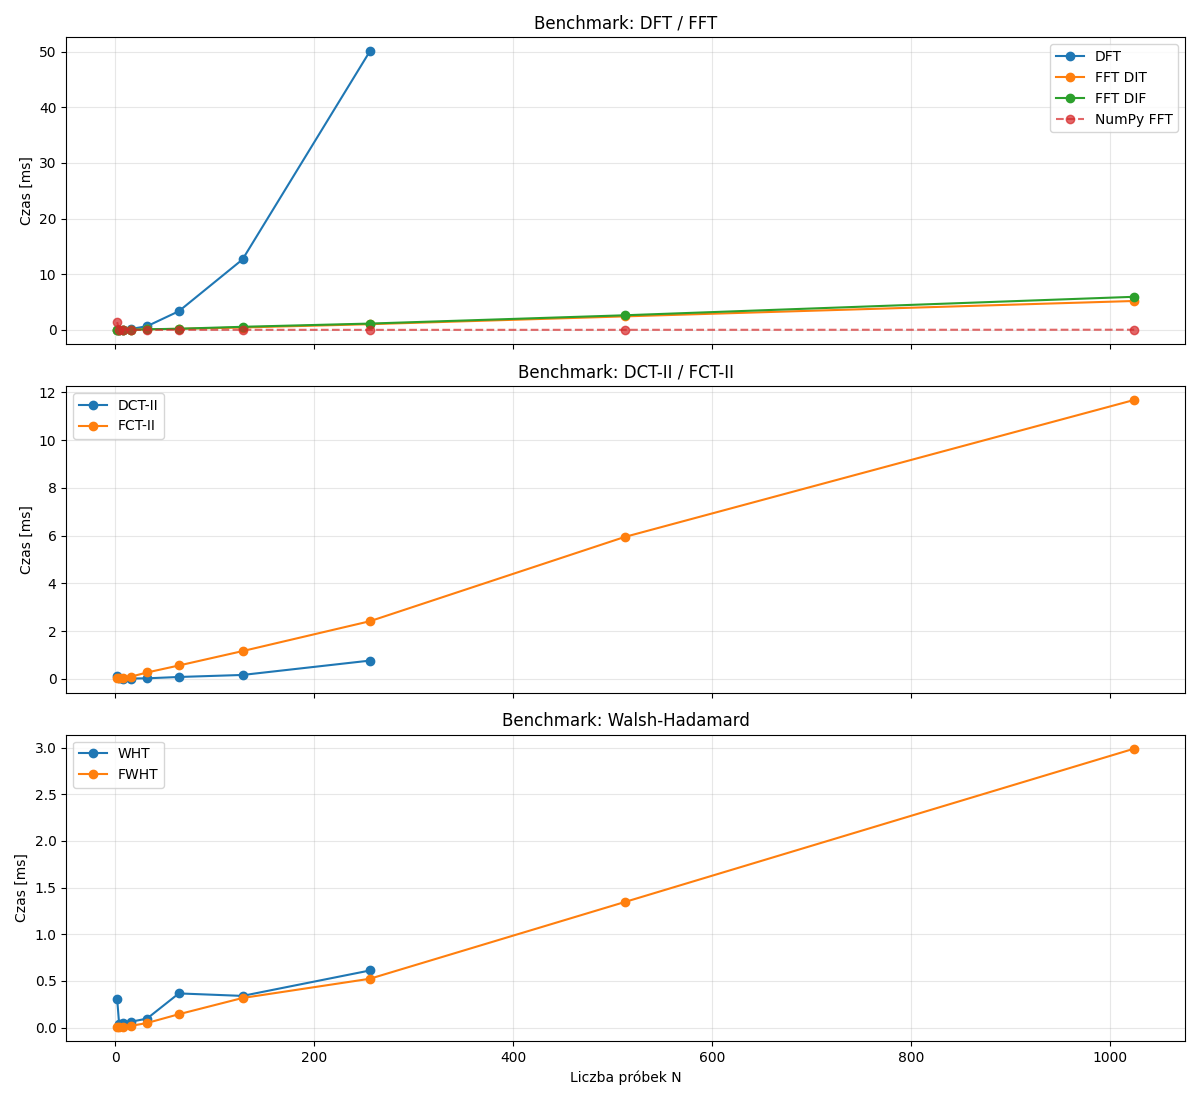
\includegraphics[width=1.0\textwidth]{img/benchmarks.png}
    \caption{Wykresy wydajności transformacji.}
    \label{fig:bench}
\end{figure}

Wyraźnie widać, że dla małych $N$ różnica jest nieznaczna, jednak powyżej $N=64$ czas DFT rośnie gwałtownie (kwadratowo), podczas gdy czas FFT rośnie w tempie zbliżonym do liniowego ($N \log N$).

\section{Wnioski}
Zaimplementowane algorytmy FFT DIT i DIF działają poprawnie, co potwierdzają błędy rzędu $10^{-14}$ w porównaniu z definicją oraz błędy rzędu $10^{-16}$ przy rekonstrukcji. Algorytmy te są drastycznie szybsze od DFT dla większych zbiorów danych, co czyni je kluczowymi w praktycznym cyfrowym przetwarzaniu sygnałów.

Dyskretna transformacja falkowa z filtrami Daubechies Db4 i Db6 również zapewnia idealną rekonstrukcję sygnału. Wykorzystanie filtrów o większej liczbie współczynników (Db6 vs Db4) pozwala na lepsze wyodrębnienie cech sygnału, ale wiąże się z nieco większym kosztem obliczeniowym na każdym poziomie dekompozycji.

Zastosowanie wizualizacji w trybach W1 i W2 pozwala na pełną analizę składowych sygnału zespolonego w dziedzinie częstotliwości, co jest niezbędne przy projektowaniu filtrów i systemów telekomunikacyjnych.

	\bibliographystyle{plain}
	\bibliography{bibliografia}
\end{document}
